\section{Proposed method}
\label{sec:proposed-method}

The proposed method is a reporting protocol for the aggregate capital figure. It takes the marginals, a correlation matrix, a set
of degrees of freedom, a level and a horizon, and returns the band of eight rows, their labels, an allocation of the aggregate
expected shortfall, the model-risk measures of the band and the results of the checks that guard the rule. Figure~\ref{fig:protocol}
shows the flow, and the subsections define each part. The protocol has no free parameter beyond the inputs: the rows are fixed by
the rule, the Monte Carlo size and the seed are stated, and nothing in the band is fitted to the outcome it is meant to describe.

\begin{figure}[htbp]
\centering
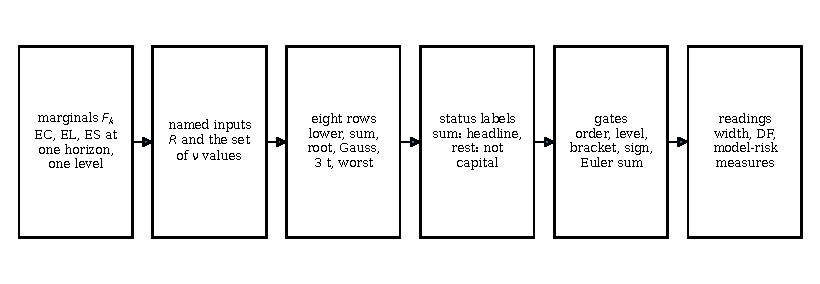
\includegraphics[width=\textwidth]{figures/protocol}
\caption{The flow of the protocol: the marginals at one horizon and one level and the named inputs (a correlation matrix and the set of degrees of freedom) produce the eight rows of the band, each row receives a status label, the checks run on the labelled band, and the readings (width, diversification factors, model-risk measures and the change under the stress) are taken from it.}
\label{fig:protocol}
\end{figure}

\subsection{The rule}
\label{sec:method-rule}

The rule has five clauses. First, an aggregate capital figure is never reported alone: it is reported with the band of aggregation
methods computed on the same marginals. Second, the band has a fixed order and a fixed content: the lower bound, the simple sum,
the square-root rule, the Gaussian copula, one $t$ copula for each degree of freedom of the named set, and the worst case, which for
the set $\{4,8,30\}$ gives eight rows (Table~\ref{tab:protocol}). Third, one horizon and one confidence level apply to every row
and to every marginal. Fourth, exactly one row, the simple sum, carries the status \emph{headline capital}; the seven other rows
carry the status \emph{information, not capital}, and so do the Euler allocation and the model-risk measures. Fifth, the inputs that
are conventions, the correlation matrices and the set of degrees of freedom, are named and labelled as conventions in the same
document, so that a reader sees which part of the band depends on a choice that no data settle.

\begin{table}[htbp]
\centering
\small
\caption{The eight rows of the band in the order in which every aggregate shows them, with the quantity each row reports, how the engine computes it and the status label it carries; only the simple sum is labelled headline capital.}
\label{tab:protocol}
\fitwidth{\begin{tabular}{rp{2.0cm}p{5.2cm}p{2.7cm}p{2.3cm}}
\toprule
\# & Row & Capital of the row & Computation & Status \\
\midrule
\relax 1 & \relax lower bound & \relax best value at risk over all couplings, less the expected losses & \relax rearrangement, outer end of the range & \relax information, not capital \\
\relax 2 & \relax simple sum (headline) & \relax sum of the marginal capitals; the comonotonic row & \relax closed form & \relax headline capital \\
\relax 3 & \relax square-root rule & $\sqrt{\mathrm{EC}^{\top}R\,\mathrm{EC}}$ with the named matrix $R$ & \relax closed form & \relax information, not capital \\
\relax 4 & \relax Gaussian copula & \relax value at risk of the sum under the Gaussian copula of $R$, less expected losses & \relax Monte Carlo, $10^6$ draws & \relax information, not capital \\
\relax 5 & $t$ copula, $\nu=4$ & \relax the same under the $t$ copula with $\nu=4$ and the matrix $R$ & \relax Monte Carlo, $10^6$ draws & \relax information, not capital \\
\relax 6 & $t$ copula, $\nu=8$ & \relax the same with $\nu=8$ & \relax Monte Carlo, $10^6$ draws & \relax information, not capital \\
\relax 7 & $t$ copula, $\nu=30$ & \relax the same with $\nu=30$ & \relax Monte Carlo, $10^6$ draws & \relax information, not capital \\
\relax 8 & \relax worst case & \relax worst value at risk over all couplings, less the expected losses & \relax rearrangement, outer end of the range & \relax information, not capital \\
\bottomrule
\end{tabular}}
\end{table}


The order is not cosmetic. It places the two sharp bounds at the ends and the simple sum next to the lower one, so that the
reader meets the extremes before the diversified figures; it also makes the structure checkable by a program, because a band whose
rows are in another order or whose labels do not follow the method is rejected.

\subsection{The rows of the band}
\label{sec:method-rows}

All rows report a capital on the basis of Equation~\ref{eq:coupling-capital}, the value at risk of the total less the sum of the
expected losses. The simple sum is $H$ of Equation~\ref{eq:ec-headline}. The square-root row combines the marginal capital figures
through the correlation matrix $R$,
\begin{equation}
b_{\mathrm{sqrt}}=\sqrt{\mathrm{EC}^{\top}R\,\mathrm{EC}},
\label{eq:sqrt-row}
\end{equation}
which equals the capital of the total when the losses are jointly elliptical with the matrix $R$ and the same family, and is
otherwise a convention. The copula rows simulate. Let $\xi\sim N(0,I_K)$, let $A$ be the Cholesky factor of $R$ so that $Z=A\xi$
has correlation $R$, and let $W\sim\chi^2_\nu$ be independent of $\xi$. The uniforms of the Gaussian and of the $t$ copula are
\begin{equation}
U_k=\Phi(Z_k),\qquad U_k=t_\nu\!\Big(Z_k\big/\sqrt{W/\nu}\Big),\qquad L_k=Q_k(U_k),
\label{eq:copula-sampling}
\end{equation}
with $\Phi$ the standard normal and $t_\nu$ the Student distribution function. With $S_i=\sum_kL_{ik}$ the total of draw $i$ and $S_{(1)}\le\dots\le S_{(n)}$ its order statistics, the capital of the row and
its Monte Carlo standard error are
\begin{equation}
b=S_{(\lceil n\alpha\rceil)}-\sum_{k=1}^K\mathrm{EL}_k ,\qquad
\mathrm{se}(b)=\frac{1}{\sqrt{B}}\,\mathrm{sd}\big(\widehat q_1,\dots,\widehat q_B\big),
\label{eq:row-capital}
\end{equation}
where $\widehat q_1,\dots,\widehat q_B$ are the sample quantiles at level $\alpha$ of $B=20$ consecutive batches of $n/B$ draws and
$\mathrm{sd}$ is the sample standard deviation. The same seed drives every simulated row, which makes the rows of one band
comparable and the band reproducible.

The two bound rows are not simulated. The lower bound is the smallest value at risk of the total over $\mathcal C$ and the worst
case is the largest, both less $\sum_k\mathrm{EL}_k$, and the rearrangement algorithm of Puccetti and R\"uschendorf
\citep{puccetti2012} computes each as a range. For the upper end, build the two $N\times K$ matrices of quantiles from the upper
tail,
\begin{equation}
\underline x_{ik}=Q_k\!\Big(\alpha+(1-\alpha)\tfrac{i-1}{N}\Big),\qquad
\overline x_{ik}=Q_k\!\Big(\alpha+(1-\alpha)\tfrac{i}{N}\Big),\qquad i=1,\dots,N ,
\label{eq:rearrangement-matrix}
\end{equation}
rearrange each column in turn to be oppositely ordered to the sum of the others, and repeat until the smallest row sum changes
by less than a tolerance $\varepsilon$. The smallest row sums of the two rearranged matrices bracket the worst value at risk
\citep{epr2013}; the lower bound is computed in the same way from the matrices on $[0,\alpha]$ with the largest row sum
minimised. The row reports the outer end of each range, the smallest end for the lower bound and the largest for the worst case,
so that the displayed interval contains the sharp one up to the accuracy of the algorithm.

\subsection{Labels and the headline}
\label{sec:method-labels}

The label of a row is a function of its method and nothing else: the simple sum is \emph{headline capital}, every other method is
\emph{information, not capital}. The functional form matters because it prevents a figure from changing status by being the
smallest, the preferred one or the most recent. A row above the headline is a true result of the method, since the value at risk
is not subadditive (Section~\ref{sec:theory}); the protocol reports it with its diversification factor above one, flags it, and
neither repairs it nor refuses it. The diversification factor $\mathrm{DF}_j=b_j/H$ is reported for every row and is the only
normalisation the band uses. The bank may choose a figure other than the simple sum as its capital, but then the choice is a
decision of the bank and not a label of the protocol, and the label of the headline stays on the simple sum. The label is carried by the document that holds the band, so that it
travels with the figure: a reader who meets a number of the band meets its status beside it. The Euler allocation and the
model-risk measures carry the same status field, and the structure check of Section~\ref{sec:results-structure} fails on a band in which one of these quantities lacks it or
carries a status that does not follow from its method.

\subsection{Allocation and model-risk measures}
\label{sec:method-allocation}

The band is accompanied by two further quantities, both labelled information. The first is the Euler allocation of the aggregate
expected shortfall of a reference copula row, here the Gaussian one. With the sample $S_i=\sum_k L_{ik}$ of $n$ draws, the
Acerbi--Tasche estimator of the expected shortfall and the contribution of risk type $k$ are
\begin{equation}
\widehat{\ES}_\alpha=\frac{1}{1-\alpha}\sum_{i=1}^n w_i S_i ,\qquad
c_k=\frac{1}{1-\alpha}\sum_{i=1}^n w_i L_{ik},\qquad \sum_{k=1}^K c_k=\widehat{\ES}_\alpha ,
\label{eq:euler}
\end{equation}
where $w_i=1/n$ for the draws above the sample quantile, a fractional weight on the draw at the quantile, and zero below
\citep{acerbi2002,tasche2008}. The sum holds by linearity for every sample, so the check on it verifies the implementation and the
bookkeeping of the allocation, not a statistical property of the dependence.

The second quantity is a pair of model-risk measures on the set of models that the band itself supplies. With $\rho_j$ the capital
of row $j$ of the band, $\rho_0$ that of the reference row (the Gaussian copula), $\overline\rho=\max_j\rho_j$ and
$\underline\rho=\min_j\rho_j$, the additive and the relative measure of Barrieu and Scandolo \citep{barrieu2015} are
\begin{equation}
\mathrm{AM}=\frac{\overline\rho}{\rho_0}-1,\qquad \mathrm{RM}=\frac{\overline\rho-\rho_0}{\overline\rho-\underline\rho}\in[0,1].
\label{eq:model-risk}
\end{equation}
$\mathrm{AM}$ is the multiplier that takes the reference figure to the worst figure of the set, and $\mathrm{RM}$ places the
reference between the two ends. The protocol adds the worst case of the expected aggregate loss over reweightings of the
sample within a budget of relative entropy, the measure of Glasserman and Xu \citep{glasserman2014}. All three are sensitivity
information for the validator: none of them is a capital figure.

\subsection{The checks}
\label{sec:method-checks}

The protocol is accompanied by nine tests, each a function that returns a light and the statistic behind it. Their acceptance
criteria are internal to the validation, not regulatory thresholds; a green light means that a statistic fell inside the criterion
and nothing more. Three tests read rows beyond the Gaussian copula. The copula-choice test computes
$\max_{\nu\in\mathcal N}\lvert b_{t,\nu}/b_{\mathrm{G}}-1\rvert$, green up to 0.05, amber up to 0.15 and red above. The bracket
test is red when a row lies outside the interval from the lower bound to the worst case. The correlation-stress test computes the
relative change of the Gaussian row between the base matrix and the stressed matrix, red when it is negative and amber above 0.10.
Six tests read the Gaussian row, the marginals or the conventions. The comparison with the simple sum and the square-root rule
tests whether the aggregate is not above the simple sum and agrees with the square-root rule within 10 percent. The sign test is
red when any diversification factor exceeds one. The consistency test counts the marginals whose horizon or level differs from the
band's and is red when the count is above zero. The additivity test compares the sum of the Euler contributions with the aggregate
expected shortfall. The agreement test compares a Monte Carlo run on elliptical marginals with the square-root row in units of its
standard error, green within three. The reference of Rosenberg and Schuermann compares the additive overestimate of the case with
the published range of 30 to 40 percent and is always green, because it is a reference and not a criterion. The tests make the
rule enforceable: a band with a missing row or a changed label does not pass its checks.

\subsection{Algorithm and complexity}
\label{sec:method-algorithm}

Algorithm~\ref{alg:band} builds the band and Algorithm~\ref{alg:rearrangement} computes the range of the bound rows.

\begin{algorithm}[htbp]
\caption{The dependence band of an aggregate.}
\label{alg:band}
\begin{algorithmic}[1]
\Require quantile functions $Q_1,\dots,Q_K$, expected losses $\mathrm{EL}_k$, capital $\mathrm{EC}_k$, matrix $R$, set $\mathcal N$, level $\alpha$, horizon $h$, draws $n$, seed $s$
\State check that $R$ is a correlation matrix, that every $\nu\in\mathcal N$ exceeds 2 and that $\mathrm{EC}_k\approx Q_k(\alpha)-\mathrm{EL}_k$ for all $k$; otherwise refuse
\State $H\gets\sum_k\mathrm{EC}_k$; $b_{\mathrm{sqrt}}\gets\sqrt{\mathrm{EC}^\top R\,\mathrm{EC}}$
\State $(\underline b,\overline b)\gets$ Algorithm~\ref{alg:rearrangement} on $Q_1,\dots,Q_K$ at level $\alpha$, less $\sum_k\mathrm{EL}_k$
\For{each family in $\{\text{Gaussian}\}\cup\{t_\nu:\nu\in\mathcal N\}$}
\State draw $n$ copula samples with seed $s$ by Equation~\ref{eq:copula-sampling}; $S_i\gets\sum_kQ_k(U_{ik})$
\State $b\gets$ sample $\alpha$-quantile of $S$ less $\sum_k\mathrm{EL}_k$; $\mathrm{se}\gets$ batch-means standard error
\EndFor
\State assemble the rows in the order lower bound, simple sum, square-root, Gaussian, $t_\nu$ for $\nu\in\mathcal N$ ascending, worst case
\State label the simple sum \emph{headline capital} and every other row \emph{information, not capital}; $\mathrm{DF}_j\gets b_j/H$
\State compute the Euler contributions of Equation~\ref{eq:euler} on the Gaussian sample and the measures of Equation~\ref{eq:model-risk}
\State run the nine tests; \Return the band, the labels, the allocation, the measures and the lights
\end{algorithmic}
\end{algorithm}

\begin{algorithm}[htbp]
\caption{Rearrangement range of the worst value at risk (upper end).}
\label{alg:rearrangement}
\begin{algorithmic}[1]
\Require quantile functions $Q_1,\dots,Q_K$, level $\alpha$, cells $N$, tolerance $\varepsilon$, sweep limit $m$, seed $s$
\State build $\underline X$ and $\overline X$ by Equation~\ref{eq:rearrangement-matrix}
\For{$X\in\{\underline X,\overline X\}$}
\State permute each column of $X$ at random under the seed; $v\gets$ smallest row sum of $X$
\Repeat
\For{$k=1$ \textbf{to} $K$}
\State rearrange column $k$ to be oppositely ordered to the sum of the other columns
\EndFor
\State $v'\gets v$; $v\gets$ smallest row sum of $X$
\Until{$\lvert v-v'\rvert<\varepsilon$ \textbf{or} $m$ sweeps}
\State $v_X\gets v$
\EndFor
\State \Return the range $(v_{\underline X},v_{\overline X})$
\end{algorithmic}
\end{algorithm}

One sweep of Algorithm~\ref{alg:rearrangement} sorts $K$ columns of $N$ cells, so it costs $O(KN\log N)$, and the number of sweeps
is small in practice (Section~\ref{sec:results-structure}); the whole bound costs about four times that, one per matrix and end.
Each copula row costs $O(nK^2)$ to draw the correlated normals, $O(nK\log G)$ to evaluate the quantile functions on a grid of
$G$ points and $O(n)$ to select the quantile, and holds $n\times K$ losses in memory, 32 megabytes for the $10^6$ draws and four
risk types of the study. The simple sum and the square-root row cost $O(K^2)$. The allocation sorts the total once, $O(n\log n)$, and the nine tests add a cost that is negligible beside it. On the
committed settings the whole band, with its four simulated rows and its two bound rows, runs in about $\bdBandSeconds$ seconds on one
workstation, of which the rearrangements take about $\bdBoundsSeconds$ seconds; the simulation dominates, and it grows linearly in $n$ while the
standard error of a row falls only as $n^{-1/2}$, which is why the band is not run with more draws than the width of the band
requires.

\subsection{Implementation}
\label{sec:method-implementation}

The protocol is implemented in the engine \texttt{riskvalidation} 1.1.0, module \texttt{aggregation.band}, whose function
\texttt{dependence\_band} returns the whole band and never a scalar. It calls \texttt{aggregation.simple} for the closed-form rows,
\texttt{aggregation.copulas} for the copula rows, \texttt{aggregation.bounds} for the rearrangement, \texttt{portfolio.euler} for
the allocation and \texttt{aggregation.model\_risk} for the measures, and the nine tests are in \texttt{validation.aggregation}
and \texttt{validation.portfolio}. A row object refuses a status that does not follow its method and a degrees-of-freedom value
on a row that is not a $t$ row. The function refuses a marginal capital that does not match its quantile function at the level of
the band, with a tolerance of one percent, so that a marginal read at another level cannot enter the band unnoticed, and it
refuses a correlation matrix that is not a correlation matrix and a set of degrees of freedom that is empty, unsorted or not
above 2. The case uses it with $n=10^6$ draws, the seed 42, a chunk of $10^5$ draws, $N=10^5$ cells and a tolerance
$\varepsilon=10^{-3}$ for the rearrangement. The committed documents of the case hold the band of each aggregate with these
settings, and every experiment of Section~\ref{sec:experimental-design} calls the same function.
